%%%%%%%%%%%%%%%%%%%%%%%%%%%%%%%%%%%%%%%%%%%%%%%%%%%%%%%%%%%%%%%%%%%%
% Grundlagen
%%%%%%%%%%%%%%%%%%%%%%%%%%%%%%%%%%%%%%%%%%%%%%%%%%%%%%%%%%%%%%%%%%%%

\chapter{Principles}
  \label{Principles}

\section{Trello}



\begin{figure}[htb]
\centering
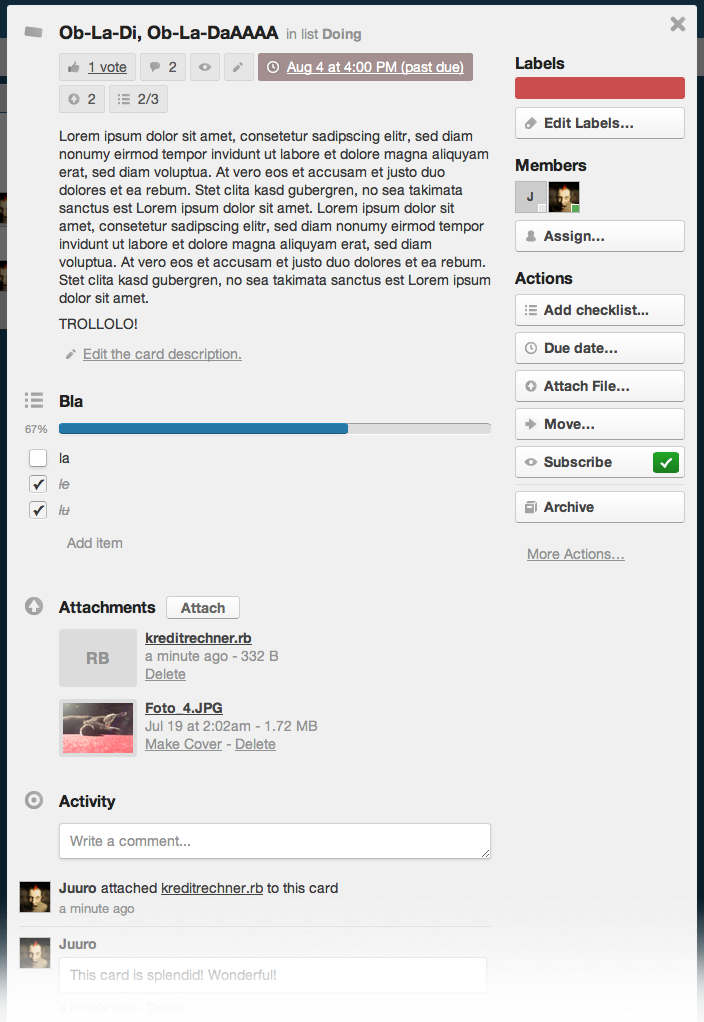
\includegraphics[width=\textwidth]{figures/trello-card}
\caption{A opened card in Trello.}
\label{fig:trello-card}
\end{figure}

\subsection{Why Trello}\index{Trello}
Trello is different from most to-do applications. It is streamlined for the purposes of small businesses. It therefore works perfectly for the needs of a university with small groups of people working on the same tasks. Trello has already proved its value for several months. The Trello website is written in HTML 5\index{HTML!5} with the use of AJAX\index{AJAX} where necessary. Trello provides an iOS\index{iOS} \cite{trello:ios} and Android\index{Android} \cite{trello:android} app, both of which are constantly evolving. So the system is state-of-the-art. In addition, the company behind Trello is not just a start-up with three employees, which is also of importance. A product of a small business, which is just based on the enthusiasm of the founders, often doesn't last long. Fog Creek Software is over ten years old and has several products.

The first aim was to see the due dates of the cards someone is assigned to in Google Calendar. Considering this, there were many other use cases for small scripts which could run as cron jobs on a server to serve several regular tasks. These scripts are described in more detail in Chapter 3.

\subsection{Trello API}\index{API}
The Trello API \nomenclature{API}{Application Programming Interface} is still in beta, but it is already very extensive. \cite{trello:docu}

\subsubsection{Authentication}
Because the scripts which are used here need access to private boards in Trello\index{Trello}, there has to be some kind of authentication. For user applications with a front end, the Trello API provides OAuth2. Because of the concept of OAuth2, however, the user is required to enter his Trello username and password. \cite{oauth} The scripts developed for this thesis are supposed to run on servers as cron jobs, so there is no user who could manually enter data. For this kind of applications, Trello provides a key/token-system. Every user has a private key with which they can generate a token. This token will be sent along every request to the Trello API. The token tells Trello which scope the request can access. While generating a token the user can specify the scope of the token and when it will expire. The possible expiration date of a token is between one day and never. In our case we will use \emph{never}. To generate a token the user has to visit a certain URL:
\texttt{
https://trello.com/1/authorize?key=SUBSTITUTEWITHYOURPRIVATEKEY \&name=My+Application\&expiration=never\&response\_type=token \&scope=read,write}
In this example the token would never expire and could read and write everything the user can access with the API. Other valid values instead of \texttt{never} for expiration would be \texttt{1day}, \texttt{30days}. \texttt{30days} is the default value. \cite{trello:gettingstarted}


\section{Ruby}\index{Ruby}
Ruby is a modern general-purpose object-oriented programming language\index{programming language}. The big difference to most other languages is that it focuses on humans rather than computers. 

Yukihiro Matsumoto\index{Matsumoto!Yukihiro}, the designer of Ruby, once said:
\begin{quote}
Ruby is simple in appearance, but is very
complex inside, just like our human body.\cite{ruby:talk}
\end{quote}

That means that Ruby\index{Ruby} is very easy to read and is intuitive\index{intuitive} for humans even though it can perform complex tasks. This is achieved with English keywords instead of brackets and curly brackets. The result of this consistent philosophy is a very easy to read language which is also very plain. Because of the English words instead of abstract characters, Ruby is easy to understand. Even non-programmers are mostly able to understand what is going on. Programmers, as a result, produce a lot fewer errors while writing the code. A wrongly spelt word is more intuitively recognisable than a missing bracket or semicolon. \cite{ruby:about} More about Ruby\index{Ruby} can be found at \url{http://www.ruby-lang.org}.

\subsection{RubyGems}\index{RubyGems}
Ruby has many methods and classes every Ruby installation\index{Ruby!installation} provides\footnote{Libraries that are included with the Ruby standard library\index{library}: \url{http://www.ruby-doc.org/stdlib-1.9.3/}}. In addition, there are hundreds of extensions\index{extensions} for special use cases – to communicate with RESTful web APIs\index{API!RESTful} for example – made by third party developers\index{developer}. In Ruby\index{Ruby}, such extensions\index{extensions} are called \emph{gems}. To manage and publish these third party libraries, there is the standard \emph{RubyGems}\index{RubyGems}. It provides a standard format for third party libraries for Ruby, a tool to manage the installation of them, and a server for distributing the gems. \cite{ruby:gemdev} Some Ruby\index{Ruby} distributions are delivered with several gems. Gems\index{Gem} can be added to an existing Ruby\index{Ruby} installation\index{installation} at any time.

To install an additional gem on a Unix\index{Unix} operating system\index{operating system}, where the Ruby standard library\index{Ruby!standard library} is installed, the following command can be used:  
\begin{center}
\texttt{gem install gemname}
\end{center}
\texttt{gemname} is here referring to the name of the respective gem\index{gem}. If the installation\index{installation} performed without errors, the gem is ready to use. \cite{ruby:gemdoc}

To use an installed gem in a Ruby\index{Ruby} script, the following code at the top of the script before the beginning of the code is necessary:

\begin{lstlisting}[aboveskip=1\baselineskip, caption=Using the gem \emph{gemname}, label=listing001]
require 'gemname'
\end{lstlisting}
Again, \emph{gemname} stands for the name of the respective gem. If any gems that are not part of the Ruby standard library\index{Ruby!standard library} are used in this script, they are listed at the beginning of the related description. Further information at \url{http://doc.rubygems.org} and \url{http://rubyforge.org/projects/rubygems/}. Additionally, \url{http://rubygems.org} is a reference book like website for Ruby gems.

\subsection{Ruby and MySQL}\label{rubymysql}\index{MySQL}\index{Ruby}
In order to access databases\index{database} in Ruby\index{Ruby}, there are additional libraries needed as the Ruby standard library doesn't support any databases. In this API wrapper, the MySQL\index{MySQL} gem is used. This gem is an API wrapper\index{API!wrapper} around the MySQL C client API. MySQL is used here because it is the most popular open source database. \cite{mysql:popularity} It is especially popular for data-handling in web applications. Therefore, the scripts described here will support MySQL\index{MySQL}.

\begin{lstlisting}[aboveskip=1\baselineskip, caption=Initialising a database connection\index{database!connection}., label=listing050]
my = Mysql.init
my.options(Mysql::SET_CHARSET_NAME, 'utf8')
my.real_connect(dbhost, dbuser, dbpassword, db)
my.query("SET NAMES utf8") (*@ \label{line050} @*)	
\end{lstlisting}

Listing \ref{listing050} above shows the initialisation of a new connection to a MySQL\index{MySQL} database with the Ruby MySQL gem. The variable \lstinline{my} is a new database handler. If the correct charset isn't set, it won't work. The host, the user, the password, and the database name should be stored in separate variables so they are easily editable. \lstinline{SET NAMES utf8} in line \ref{line050} of listing \ref{listing050} is a first execution of a MySQL query\index{MySQL!query}. It tells the server the charset name of future connections. In this example, the server expects all future queries as UTF8 \nomenclature{UTF-8}{8-Bit UCS Transformation Format}\nomenclature{UCS}{Universal Character Set} charset.

MySQL statements\index{MySQL!statement} can be executed directly or as \emph{prepared statements}. The example in line \ref{line050} of  \ref{listing050} is a normal statement which is executed directly. Listing \ref{listing051} shows a longer example. 

\begin{lstlisting}[aboveskip=1\baselineskip, caption=Example for a directly executed MySQL query., label=listing051]
response = my.query(" 
	SELECT fieldname1 (*@ \label{line0305} @*)
	FROM tablename 
	WHERE  fieldname2=value
	AND fieldname3=value (*@ \label{line031} @*)
")
response.each do |row|
	puts row (*@ \label{line032} @*)
end
\end{lstlisting}

The MySQL statement\index{MySQL!statement} between line \ref{line0305} and \ref{line031} responds with data, so the result of the query must somehow be read. The response of a \lstinline{SELECT} statement is an array of rows from the given table. To get the lines of the response table, the \lstinline{each} method is used to iterate through the array and print each row.

\begin{lstlisting}[aboveskip=1\baselineskip, caption=\texttt{joomlaMultiple.rb} usage., label=listing029]
statement = my.prepare("
	INSERT INTO tablename (
		fieldname1,
		fieldname2
	) 
	VALUES (
		?,
		?
	)
")
statement.execute value1, value2 (*@ \label{line052} @*)
statement.execute othervalue1, othervalue2 (*@ \label{line053} @*)
\end{lstlisting}

The listing above shows how the MySQL library\index{MySQL!library} for Ruby\index{Ruby} handles prepared statements. The big difference to directly executed statements are the wildcards in the \lstinline{VALUES} part. It's more like a template for a statement. Although the statement doesn't contain all required values, it is sent to the underlying DBMS of MySQL. The DBMS\index{DBMS} can already perform query optimisation\index{query optimisation} on this statement template. To fill in the actual values, the statement must be executed with the \lstinline{execute} method. The lines \ref{line052} and \ref{line053} are two executions of the specified statement. In this step, the wildcards are replaced by the actual values. The DBMS\index{DBMS} performs additional query optimisation\index{query optimisation} if needed. Sometimes, query optimisation depends on the values of the fields. Prepared statements\index{prepared statements} can be executed multiple times. That saves performance, because the initial query optimisation must be performed only once. In addition, prepared statements\index{prepared statements} are safer than directly executed statements. Because the DBMS\index{DBMS} processes the MySQL\index{MySQL} code separately to the actual data, it can distinguish between valid and invalid data. The DBMS checks every given value before writing it to the database. Because of that, SQL injection\index{SQL!injection} isn't possible with prepared statements. For every MySQL statement that writes data to the database\index{database}, it is therefore reasonable to use prepared statements\index{prepared statements}. \cite{mysql:rubydoc}

\subsection{Error handling}\index{error handling}
Because these scripts access mostly web servers, sometimes multiple in a single execution, error handling\index{error handling} is essential. There are many reasons why an API call\index{API!call} can't be executed properly, but the connection is a common reason. It's very useful to the user if  they know the reason why a script failed to execute. Error handling ensures, that the script posts an error message, at least. So the user has a chance to find out what's the reason for the problem and if he can do anything about it.

Error handling in Ruby is realised with \lstinline{begin} blocks. A \lstinline{begin} block is like an \lstinline{if} expression but for \emph{exceptions}\index{exception}. 

\begin{lstlisting}[aboveskip=1\baselineskip, caption=Error handling with \lstinline{begin} blocks., label=listing042]
begin
	my = Mysql.init
	my.real_connect(dbhost, dbuser, dbpassword, db)
rescue => e
	puts e.message
else  (*@ \label{line036} @*)
	puts "It works!"
ensure
	mysql.close if mysql
end
\end{lstlisting}

A \lstinline{begin} block has several sections. The first section is the \lstinline{begin} section. Here, the code to check is executed. The example in listing \ref{listing042} shows a simple database connection. With the \lstinline{begin} block around it, Ruby\index{Ruby} checks if any exceptions\index{exception} occur while executing this code. If there indeed are exceptions, the \lstinline{rescue} section comes to help out. The error is stored in the variable \lstinline{e}. At least the message can be printed here, to inform the user. A \lstinline{begin} block may contain multiple \lstinline{rescue} sections. It's possible to specify special types of exceptions, so corresponding actions can be performed. 

\begin{lstlisting}[aboveskip=1\baselineskip, caption=\texttt{joomlaMultiple.rb} usage., label=listing043]
rescue Mysql::Error => e
\end{lstlisting}

In listing \ref{listing043} the \lstinline{Mysql::Error} class is specified. In this \lstinline{rescue} section only exception\index{exception} of this class will be handled.

An \lstinline{else} section in a \lstinline{begin} block like in line \ref{line036} of listing \ref{listing042}, is allowed only if there are one or more \lstinline{rescue} blocks. It is executed if there are no exceptions. The last section is the \lstinline{ensure} block. It is executed no matter whether there is an exception\index{exception} or not. In the example, the initialised database\index{database} connection is closed. This section is supposed to finish the execution of the whole block. \cite{skorks}

\section{REST}\nomenclature{REST}{Representational State Transfer}
The Trello API is a \emph{RESTful}\index{RESTful} web API. That means that the API is conform to the REST design model. REST is a common style of software architecture for distributed systems. It is built on four of the HTTP request methods\index{HTTP!request method}: GET, POST, PUT and DELETE. An implementation of a RESTful\index{RESTful} web service follows four basic design principles:
\begin{itemize}
	\item Use HTTP\nomenclature{HTTP}{Hyper Text Transfer Protocol} methods explicitly.
	\item Be stateless.
	\item Expose directory structure-like URIs\nomenclature{URI}{Uniform Resource Identifier}.
	\item Transfer XML\nomenclature{XML}{Extensible Markup Language} , JSON\nomenclature{JSON}{JavaScript Object Notation}, or both.
\end{itemize}
\cite{rest}

Following these conventions a GET URL of a RESTful\index{RESTful} web service looks like this:
\begin{center}
\texttt{https://api.trello.com/1/cards/4fc8dd3e1b9ecf0c3571902f? key='PRIVATEKEY\&token=TOKEN}
\end{center}
This is a GET request to get a specific card with the ID \texttt{4fc8dd3e1b9ecf0c3571902f}. If this URL\nomenclature{URL}{Uniform Resource Locator} is visited in a browser\index{browser} (with correct \emph{key} and \emph{token}), the browser will show plain JSON\index{JSON}. In order for Ruby to be able to work with it, it must somehow capture this data. To fulfill the requirements of REST in Ruby, there are several gems. Here the RestClient gem is used. This GET request executed with the RestClient gem in Ruby looks like \ref{listing019}.

\begin{lstlisting}[aboveskip=1\baselineskip, caption=GET request using RestClient., label=listing019]
member = RestClient.get('https://api.trello.com/1/cards/4fc8dd3e1b9ecf0c3571902f?key='+$key+'&token='+$token)
pp JSON.parse(member)
\end{lstlisting}

In comparison to the open-uri library, which is included in the Ruby standard library, using RestClient\index{RestClient} results in much cleaner code, especially when it comes to POST requests.

\begin{lstlisting}[aboveskip=1\baselineskip, caption=POST request using RestClient., label=listing009]
response = RestClient.post(
	'https://api.trello.com/1/boards',
	:name => board['name'], 
	:desc => board['desc'],
	:key => $key,
	:token => $token
)
\end{lstlisting}

\begin{lstlisting}[aboveskip=1\baselineskip, caption=POST request with open-uri., label=listing010]
uri = URI('https://api.trello.com/1/boards')
req = Net::HTTP::Post.new(uri.path)

req.set_form_data(
	'name' => board['name'], 
	'desc' => board['desc'],
	'key'=>$key,
	'token'=>$token
)

Net::HTTP.start(uri.host, uri.port, :use_ssl => uri.scheme == 'https') do |http|
	response = http.request(req)
end
\end{lstlisting}

Listing \ref{listing009} and listing \ref{listing010} show the very same API call. But \ref{listing009} is realised with RestClient and listing \ref{listing010} with open-uri\index{open-uri}. Not only is the open-uri\index{open-uri} code much longer, but open-uri\index{open-uri} also doesn't detect the correct scheme from the given URI. If the call should be performed in HTTPS, this has to be set explicitly. This implies that for the handling of RESTful\index{RESTful} web services, RestClient is the better choice.


\section{JSON}\index{JSON}\label{jsonsec}
All the responses of Trello\index{Trello} API\index{API} calls are in the JSON\footnote{RFC\nomenclature{RFC}{Request For Comments} document for JSON: The application/json Media Type for JavaScript Object Notation (JSON)  \url{http://www.ietf.org/rfc/rfc4627.txt}} format, which is a subset of the JavaScript programming language. Despite its relation to JavaScript, it is language independent. JSON is a data-interchange format like XML, but it is built on two structures. One is a list of key/value pairs. In most programming languages, this is realised as a hash, struct, object, or associative array. The other structure is an ordered list of values. This is realised as an array, list, vector, or sequence in popular programming languages. In JSON itself, these structures are called \emph{object} and \emph{array}. Objects start and end with curly brackets. Each key is followed by a colon and the key/value pairs are separated by commas. Arrays start and end with squared brackets, the values are again separated by commas. Both can be arbitrarily nested. Every time one of the scripts saves content to any other place than Trello, it is also in the JSON\index{JSON} format in order to guarantee easy compatibility with Trello. JSON\index{JSON} can be saved in files, too. A JSON\index{JSON} file has the suffix \texttt{.json}. \cite{json}

\begin{lstlisting}[aboveskip=1\baselineskip, caption=JSON example., label=listing054]
{
    "id": "4eea4ffc91e31d1746000046",
    "name": "Example Board",
    "desc": "This board is used in the API examples",
    "lists": [{
        "id": "4eea4ffc91e31d174600004a",
        "name": "To Do Soon"
    }, {
        "id": "4eea4ffc91e31d174600004b",
        "name": "Doing"
    }, {
        "id": "4eea4ffc91e31d174600004c",
        "name": "Done"
    }]
}
\end{lstlisting}

In listing \ref{listing054}, a JSON example is shown. This is the response of

\begin{center}
\texttt{https://api.trello.com/1/boards/4eea4ffc91e31d1746000046? lists=open\&list\_fields=name,desc\&key=PRIVATEKEY\&token=TOKEN}
\end{center}

The JSON in listing \ref{listing054} starts with a curly bracket. That means the uppermost structure is an object. Here are a few key/value pairs like \texttt{"id": "4eea4ffc91e31d1746000046"}. The key \texttt{"list"} has an array as value, so their value is in squared brackets. Each element of the array is, again, an object.

To process the received JSON, Ruby needs to parse it first. For that purpose, there is the a gem simply called \emph{JSON}. It parses the JSON with the 

\begin{center}
\lstinline{JSON.parse(receivedJson)} 
\end{center}
command, where \lstinline{receivedJson} is a variable that contains the plain JSON received from the Trello API with a GET request. After the parsing, the JSON objects are now represented as Ruby hashes and the JSON arrays as Ruby arrays. To post content to the Trello API, it has to be in JSON\index{JSON}, too. There is another method of the JSON class in Ruby which generates JSON from Ruby hashes and arrays. 

\begin{center}
\lstinline{JSON.generate(hashBoards)} 
\end{center}

The result is a valid JSON formatted string, ready to be written to a JSON file or sent to an API.